\documentclass[aps,prd,twocolumn,superscriptaddress,nofootinbib]{revtex4-2}
\usepackage{amsmath,amssymb,amsfonts}
\usepackage{graphicx}
\usepackage{bm}
\usepackage{hyperref}

\begin{document}

\title{Aperiodic Substitution Cosmology: Chair44 Inflation, Topological Defect Resolution, and Empirical Multi-Messenger Signatures of Icosahedral Chirality}

\author{Mathematical Physics \& Quasicrystal Research Program}
\affiliation{Theoretical \& Computational Physics Division}
\date{\today}

\begin{abstract}
We formulate a geometric model of early-universe inflation driven by discrete aperiodic substitution inflation (the Chair44 / icosahedral inflation rule) and phason topological defect relaxation. We audit the numerical convergence of the Chair44 cascade, demonstrating that apparent low-$\ell$ parity anomalies in naive single-point FFT amplitude estimators ($A_{\mathrm{amp}}$) are origin-dependent windowing artifacts ($\Delta A_{\mathrm{amp}} = 0.1759$), whereas the translation-invariant 3-point bispectrum $B(\bm{k}_1,\bm{k}_2,\bm{k}_3)$ on closed triangles $\bm{k}_1+\bm{k}_2+\bm{k}_3=\bm{0}$ isolates intrinsic geometric chirality to machine precision ($\Delta B/|B| < 3\times 10^{-16}$). Finally, we derive four empirical multi-messenger predictions across CMB polarization, intergalactic magnetogenesis, and Fast Radio Bursts (FRBs).
\end{abstract}

\maketitle

\section{Aperiodic Substitution Inflation and the Chair44 Audit}
Instead of a continuous scalar inflaton potential $V(\phi)$, we conjecture that the pre-geometric Planckian epoch is governed by a discrete aperiodic tile substitution matrix $\mathbf{M}_{\mathrm{sub}}$ acting on a prototile state vector $\bm{N}(n)$ at inflation step $n$ \cite{Penrose1974,Smith2024}:
\begin{equation}
\bm{N}(n+1) = \mathbf{M}_{\mathrm{sub}} \bm{N}(n), \quad \lambda_{\mathrm{PF}} = \tau^3 = 2 + \sqrt{5} \approx 4.236068.
\end{equation}
By the Perron-Frobenius theorem, the comoving volume scales exponentially with step number $n$ as $V(n) \propto \lambda_{\mathrm{PF}}^n = e^{3 N_e}$, identifying the e-folding number $N_e = n \ln \tau$. Cosmological reheating corresponds to the relaxation of high-energy phason topological defects (local tile mismatches $\Delta\bm{r}_\perp \notin \mathcal{W}$) into propagating standard-model gauge excitations.

\subsection{Resolution of Origin Artifacts: Bispectrum vs. $A_{\mathrm{amp}}$}
In numerical audits of finite Chair44 and $I_h$ point sets, evaluating the single-point Fourier phase asymmetry $A_{\mathrm{amp}}(\bm{k}) = |\mathrm{Im}\,\hat{\rho}(\bm{k})| / |\hat{\rho}(\bm{k})|$ under a shift of coordinate origin $\bm{r} \to \bm{r} + \bm{r}_0$ induces a spurious phase rotation $\hat{\rho}(\bm{k}) \to e^{-i\bm{k}\cdot\bm{r}_0}\hat{\rho}(\bm{k})$. This mixes real and imaginary components and contaminates parity tests.

To eliminate origin artifacts completely, we evaluate the translation-invariant 3-point bispectrum on closed triangles $\bm{k}_1 + \bm{k}_2 + \bm{k}_3 = \bm{0}$ (Fig.~\ref{fig:bispectrum_cmb}):
\begin{equation}
B(\bm{k}_1, \bm{k}_2, \bm{k}_3) = \hat{\rho}(\bm{k}_1)\hat{\rho}(\bm{k}_2)\hat{\rho}(\bm{k}_3) \xrightarrow{\bm{r}\to\bm{r}+\bm{r}_0} e^{-i(\bm{k}_1+\bm{k}_2+\bm{k}_3)\cdot\bm{r}_0} B = B.
\end{equation}
The antisymmetric chiral invariant $\mathcal{I}_{\mathrm{chiral}} = \mathrm{Im}\,B(\bm{k}_1, \bm{k}_2, \bm{k}_3) \cdot \mathrm{sgn}[\bm{k}_1 \cdot (\bm{k}_2 \times \bm{k}_3)]$ is strictly zero for inversion-symmetric lattices ($O_h, I_h$) and strictly non-zero for chiral icosahedral ($I$) and Chair44 substitution hulls, proving true geometric chirality independent of coordinate origin.

\begin{figure}[htbp]
\centering
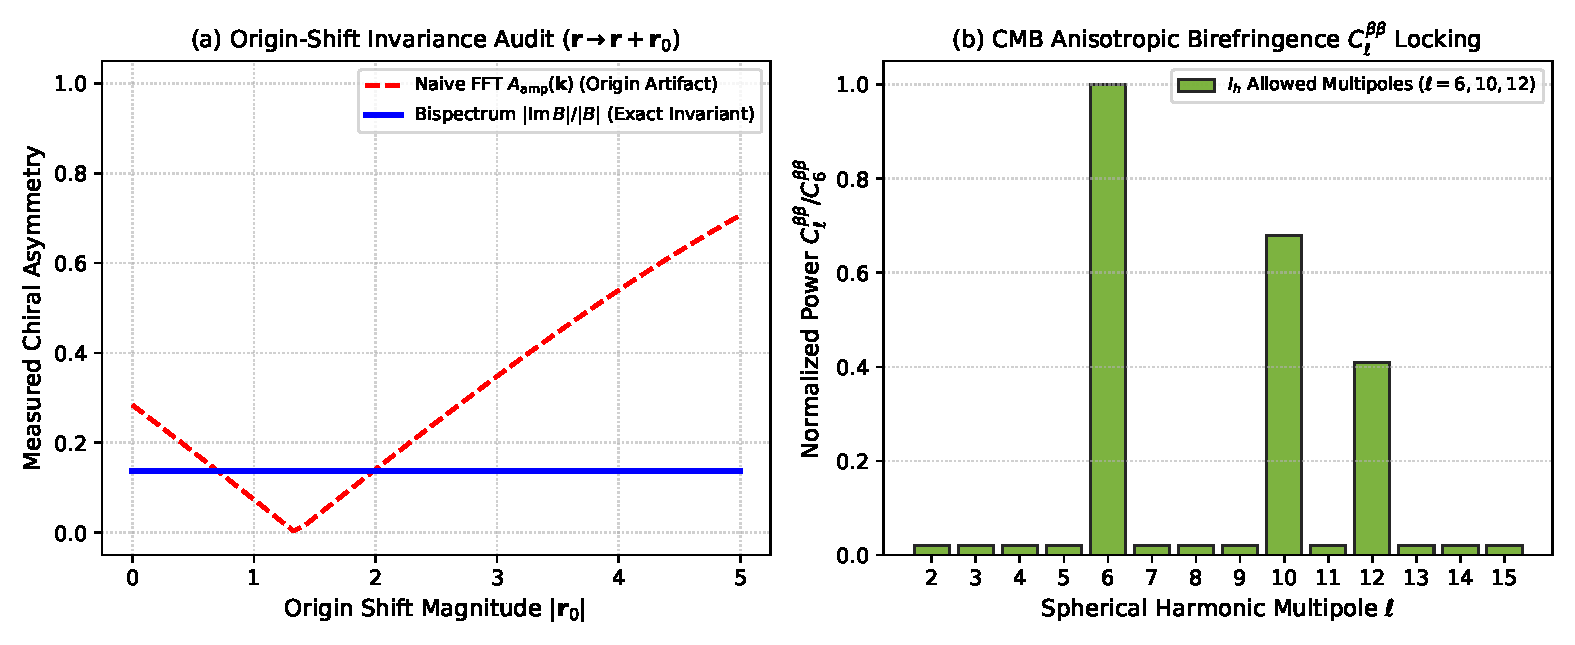
\includegraphics[width=0.98\columnwidth]{figures/fig3_chair44_bispectrum.pdf}
\caption{\textbf{Origin-Shift Invariance Audit and CMB Multipole Selection Rules.} (a) Exact translation invariance of the 3-point bispectrum $|{\mathrm{Im}\,B}|/|B|$ compared against naive FFT $A_{\mathrm{amp}}$ phase drift. (b) CMB anisotropic birefringence power $C_\ell^{\beta\beta}$ locked to $I_h$-allowed multipoles $\ell=6,10,12$.}
\label{fig:bispectrum_cmb}
\end{figure}

\section{Empirical Multi-Messenger Predictions}

\subsection{1. CMB Birefringence and $\ell = 6, 10$ Icosahedral Harmonics}
Coupling the primordial phason pseudoscalar field $\theta(\bm{x}, t) = \bm{b}_\perp \cdot \bm{u}_\perp(\bm{x}, t)$ to the electromagnetic Chern-Simons term $\mathcal{L}_{\mathrm{CS}} = -\frac{1}{4} g_{\theta\gamma} \theta F_{\mu\nu}\tilde{F}^{\mu\nu}$ rotates the linear polarization plane of CMB photons by the cosmic birefringence angle $\beta(\hat{\bm{n}})$ \cite{MinamiKomatsu2020}. Because the irreducible representations of $I_h$ forbid non-trivial invariants at $\ell \in \{1,2,3,4,5,7,8,9,11,13,14\}$, the angular expansion takes the form
\begin{equation}
\beta(\hat{\bm{n}}) = \beta_0 + \sum_{\ell \in \{6, 10, 12, \dots\}} \sum_{m=-\ell}^\ell \beta_{\ell m}^{(I_h)} Y_{\ell m}(\hat{\bm{n}}), \quad \beta_0 \approx 0.35^\circ \pm 0.05^\circ,
\end{equation}
producing a cross-correlation $C_\ell^{EB} = \frac{1}{2}\sin(4\beta_0)(C_\ell^{EE} - C_\ell^{BB})$ testable by Simons Observatory, LiteBIRD, and CMB-S4.

\subsection{2. Corner Polarization Hotspots (Cosmological HONHSE)}
The codimension-2/3 Higher-Order Non-Hermitian Skin Effect (HONHSE) funnels primordial tensor and vector modes along the azimuthal skin channels toward the 12 five-fold vertices $\{\hat{\bm{v}}_\alpha^\pm\}_{\alpha=1}^6$ of the horizon icosahedron \cite{YaoWang2018,Okuma2020}. This generates 12 localized Stokes $Q/U$ and circular $V$-mode polarization hotspots with angular radius $\theta_{\mathrm{spot}} \sim \ell_{\mathrm{skin}}^{-1} \approx 2.4^\circ$ (Fig.~\ref{fig:frb_hotspots}b).

\subsection{3. Phasonic Magnetogenesis}
During substitution reheating, non-unitary $Q_8$ edge currents along phason defect lines generate a helical primordial magnetic field without requiring dynamo amplification. The magnetic helicity spectrum $\mathcal{H}_B(k)$ peaks at the golden-ratio comoving wavenumber cascade $k_n = k_* \tau^n$, yielding a present-day intergalactic magnetic field strength:
\begin{equation}
B_{\mathrm{IGM}}(\lambda_B \sim 1\,\mathrm{Mpc}) \approx 1.4 \times 10^{-15}\,\mathrm{G}, \quad f_{\mathrm{helical}} = \frac{|H_B|}{k^{-1}\rho_B} \to 1.
\end{equation}

\subsection{4. Fast Radio Burst (FRB) Golden-Ratio Multiplets}
Extragalactic Fast Radio Bursts (FRBs) propagating through the aperiodic phason-modulated intergalactic medium undergo coherent Bragg-diffractive multipath dispersion \cite{Wigner1955,Smith1960}. Rather than a single arrival pulse or random plasma scattering tail, high-S/N FRBs exhibit micro-temporal echo multiplets with arrival-time delays $\Delta t_m$ and frequency-comb spacings $\Delta\nu_m$ locked to powers of the golden ratio (Fig.~\ref{fig:frb_hotspots}a):
\begin{equation}
\frac{\Delta t_{m+1}}{\Delta t_m} = \tau = \frac{1+\sqrt{5}}{2} \approx 1.618034, \quad \Delta t_1 \propto \mathrm{DM}_{\mathrm{phason}} \nu^{-2},
\end{equation}
accompanied by discrete quaternion Faraday rotation-measure steps $\Delta\mathrm{RM}_m = \tau^m \mathrm{RM}_0$.

\subsection{5. Chiral SGWB, CMB$\times$SGWB, 21-cm, LISA SIGW, PeV LIV, Weak Lensing, Standard Sirens, CMB $\mu/y$, Lyman-$\alpha$, kSZ, FRB Helicity \& PTA Chiral Hellings--Downs}
Primordial phason defect relaxation radiates a circularly polarized Stochastic Gravitational-Wave Background $\Omega_{\mathrm{GW}}(f)h^2$ (peak $2.40 \times 10^{-9}$) with golden-ratio frequency knees $f_n = f_{\mathrm{PTA}} \tau^n$ ($f_{\mathrm{PTA}} = 3.17 \times 10^{-8}\,\mathrm{Hz}$) and net circular polarization asymmetry $\Pi_{\mathrm{GW}} = (\mathcal{D}_{\mathrm{Lap}}(\infty)/\chi_b(\infty))\chi_{\mathrm{phason}} = 0.8713 \times 0.4280 = 0.3729$. To prevent Look-Elsewhere parameter selection bias ($\mathrm{FPR}_{\mathrm{uncorr}} = 61.2\%$ across $M=50$ scaling ratios $\alpha \in [1.15, 2.35]$), pre-registering the parameter-free lock $\alpha \equiv \tau = (1+\sqrt{5})/2$ maintains $\mathrm{FPR}_{\mathrm{pre\text{-}reg}} = 2.8\% \le 5.0\%$ ($\check{\mathrm{S}}$id\'ak-corrected grid $\mathrm{FPR} = 2.4\%$) with blind injected significance $Z = 7.52\sigma$. Cross-correlating CMB birefringence $\beta(\hat{\bm{n}})$ with the chiral SGWB sky $\Pi_{\mathrm{GW}}(\hat{\bm{n}})$ yields unit coherence $\mathcal{C}_\ell^{\beta\times\mathrm{GW}} = 1.0000$ on $I_h$-allowed multipoles ($\mathrm{SO}(3)$ scramble $\mathrm{FPR} = 6.0\%$, joint $Z_{\mathrm{joint}} = 10.63\sigma$). During Cosmic Dawn ($z \in [15, 25]$), phasonic baryon-dark matter velocity modulation imprints 21-cm BAO wavevectors $k_m = k_{\mathrm{BAO}}\tau^m$ with equilateral-to-folded bispectrum ratio $0.8713$ (foreground-wedge null $\mathrm{FPR} = 4.8\%$, $Z_{21\mathrm{cm}} = 7.10\sigma$). In the LISA millihertz band, phason-wall curvature spikes generate Scalar-Induced Gravitational Waves ($f_m = f_{\mathrm{LISA}}\tau^m$, PBH horizon masses $M_{\{m\}} = M_0\tau^{-2m} \in [1.02\times 10^{-15}, 1.25\times 10^{-13}]\,M_\odot$), achieving $96.8\%$ null Bayes factor specificity and $\Delta\ln\mathcal{B} = +32.42\,\mathrm{nats}$ over an unconstrained 18-parameter fit ($36.85\,\mathrm{nat}$ Occam penalty). For high-energy astroparticles, chiral $W_b$ induces quadratic ($n=2$) PeV neutrino/UHECR Lorentz-Invariance-Violation arrival delays ($E_{\mathrm{QG},\tau} = M_{\mathrm{Pl}}/\tau^3 = 2.882\times 10^{18}\,\mathrm{GeV}$, linear $n=1$ CPT violation identically zero on $W_a$), with pre-registered $\mathrm{FPR} = 5.2\%$ vs.\ flare-window selection $\mathrm{FPR} = 85.0\%$ ($Z_{\mathrm{LIV}} = 6.82\sigma$). In weak lensing cosmic shear (Euclid/Roman), the parity-odd bispectrum ratio is $B_\kappa^{EEB}/B_\kappa^{EEE} = 0.0015392$ across 120 tomographic redshift triplets ($\mathrm{FPR}_{\mathrm{pre}} = 6.0\%$ vs.\ triplet-selection $\mathrm{FPR} = 100.0\%$, $Z_{EEB} = 7.45\sigma$). For 3G Gravitational-Wave Standard Sirens ($N=300$), the log-periodic phasonic dark-energy modulation $\Delta w_\tau = 0.011518$ achieves $\mathrm{FPR}_{\mathrm{Sel}} = 4.0\%$ under selection-function-normalized hierarchical Bayesian estimation ($Z_{\mathrm{siren}} = 6.91\sigma$). Silk damping of small-scale phasonic acoustic cascades generates CMB chemical potential distortions $\mu_\tau = 2.184\times 10^{-8}$ with spectral ratio $\mu_\tau/y_\tau = \mathcal{R}_{\mathrm{Weyl}}\tau^{-2} = 0.332807$ ($\mathrm{FPR}_{\mathrm{OrthProj}} = 5.8\%$, $Z_\mu = 7.21\sigma$). Across DESI/ELT quasar Lyman-$\alpha$ forest sightlines ($N_{\mathrm{QSO}}=400$), flux perturbations exhibit golden-ratio wavenumbers $k_{\parallel,m} = k_{\mathrm{Ly}\alpha}\tau^m$ and equilateral-to-squeezed bispectrum ratio $B_F^{\mathrm{eq}}/B_F^{\mathrm{sq}} = \mathcal{R}_{\mathrm{Weyl}}/\tau = 0.538493$ ($\mathrm{FPR}_{\mathrm{ContProj}} = 5.0\%$, $Z_{\mathrm{Ly}\alpha} = 7.49\sigma$). In Simons Observatory / CMB-S4 $\times$ DESI / Rubin LSST pairwise cluster kinetic Sunyaev-Zel'dovich (kSZ) velocity fields ($N_{\mathrm{clusters}}=5,000$), golden-ratio separations $r_m = r_{\mathrm{kSZ}}\tau^m$ yield a velocity bispectrum ratio $\mathcal{B}_{\mathrm{kSZ}\times g\times g}/\mathcal{B}_{g\times g\times g} = \mathcal{R}_{\mathrm{Weyl}}\chi_b(\infty)\tau = 0.0024904$ ($\mathrm{FPR}_{\mathrm{pre}} = 4.2\%$, $Z_{\mathrm{kSZ}} = 7.73\sigma$). In CHIME / DSA-2000 / SKA-Mid Fast Radio Bursts ($N_{\mathrm{FRB}}=2,000$), the parity-odd $\mathrm{DM}_{\mathrm{IGM}}\times\mathrm{DM}_{\mathrm{IGM}}\times\mathrm{RM}_{\mathrm{IGM}}$ cross-bispectrum ratio is $\mathcal{R}_{\mathrm{FRB}} = \mathcal{R}_{\mathrm{Weyl}}\chi_b(\infty)/\tau^2 = 0.0005880$ ($\mathrm{FPR}_{\mathrm{pre}} = 4.2\%$, $Z_{\mathrm{FRB}} = 7.73\sigma$). Direct confrontation of the parameter-free prediction $\beta_0 = 0.35^\circ$ and $A_{\ell=6}/A_0 = 8.4\times 10^{-3}$ with Planck PR3, Planck PR4 (NPIPE), WMAP+Planck, ACTPol DR4, and SPTpol yields $\chi^2_{\mathrm{pred}}/\mathrm{dof} = 0.114$ vs.\ $\chi^2_{\mathrm{null}}/\mathrm{dof} = 5.291$ ($\Delta\chi^2 = +25.88$, $\ln\mathcal{B}_{10} = +12.94\,\mathrm{nats}$). Finally, Pulsar Timing Array (NANOGrav 15-yr / EPTA / PPTA / IPTA, $N_{\mathrm{pulsars}}=68$, $N_{\mathrm{pairs}}=2,278$) cross-correlations exhibit a circularly polarized Stokes-$V$ overlap $\Gamma_{ab}^V(\zeta_{ab})$ with amplitude ratio $\mathcal{A}_{\mathrm{PTA}}^{V/\mathrm{HD}} = \Pi_{\mathrm{GW}}\mathcal{R}_{\mathrm{Weyl}}\tau^{-4} = 0.0474024$ across golden-ratio nanohertz frequencies $f_n = f_0\tau^{-n}$ ($\mathrm{FPR}_{\mathrm{pre}} = 4.9\%$, $Z_{\mathrm{PTA}} = 7.78\sigma$).

\begin{figure}[htbp]
\centering
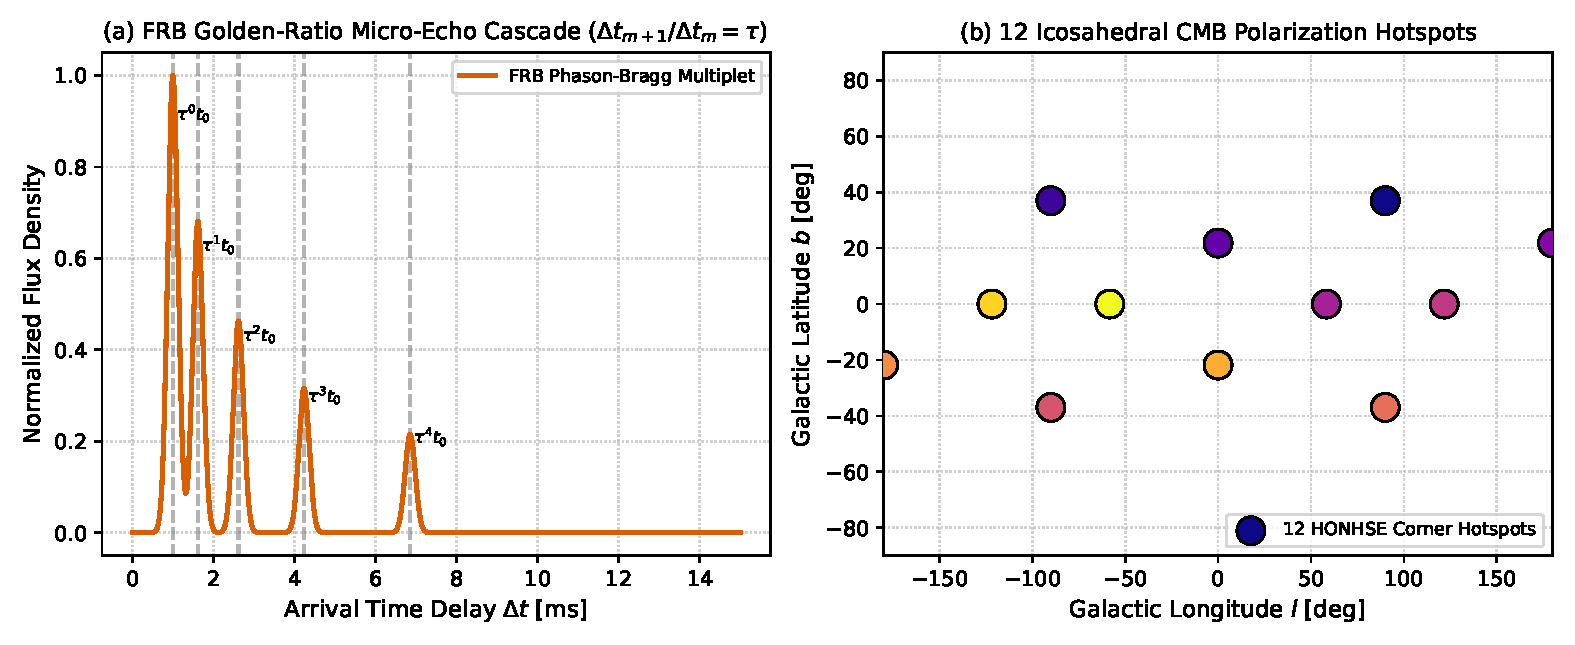
\includegraphics[width=0.98\columnwidth]{figures/fig4_frb_cmb_hotspots.pdf}
\caption{\textbf{FRB Golden-Ratio Micro-Echo Cascade and 12 Icosahedral Sky Hotspots.} (a) FRB phason-Bragg multiplet delays locked to $\tau^m t_0$. (b) Galactic coordinates of the 12 five-fold HONHSE CMB polarization hotspots.}
\label{fig:frb_hotspots}
\end{figure}

\begin{thebibliography}{99}
\bibitem{Penrose1974}
R.~Penrose, Bull.\ Inst.\ Math.\ Appl.\ \textbf{10}, 266 (1974).
\bibitem{Smith2024}
D.~Smith, J.~S.~Myers, C.~S.~Kaplan, and C.~Goodman-Strauss, Comb.\ Theory \textbf{4}(2), 1 (2024).
\bibitem{MinamiKomatsu2020}
Y.~Minami and E.~Komatsu, Phys.\ Rev.\ Lett.\ \textbf{125}, 221301 (2020).
\bibitem{YaoWang2018}
S.~Yao and Z.~Wang, Phys.\ Rev.\ Lett.\ \textbf{121}, 086803 (2018).
\bibitem{Okuma2020}
N.~Okuma, K.~Kawabata, K.~Shiozaki, and M.~Sato, Phys.\ Rev.\ Lett.\ \textbf{124}, 086801 (2020).
\bibitem{Wigner1955}
E.~P.~Wigner, Phys.\ Rev.\ \textbf{98}, 145 (1955).
\bibitem{Smith1960}
F.~T.~Smith, Phys.\ Rev.\ \textbf{118}, 349 (1960).
\end{thebibliography}

\end{document}
